\label{Effective potential}
This section is based on \cite{Peskin:IntroQFT,weinberg_1995,weinberg_1996_vol2} (Schwarz).
The ground state partition function is given by
\begin{equation}
    Z = \lim_{T\rightarrow \infty} \braket{\Omega, T}{-T, \Omega}
    = \lim_{T\rightarrow \infty} \inner{\Omega}{ e^{-2iHT} }{\Omega}
    = \int \D \pi \D \varphi \, \exp{ i \int \dd^4 x \, \left(\pi \dot \varphi - \He[\pi, \varphi]\right) },
\end{equation}
where $\ket{\Omega}$ is the vacuum of the theory~\cite{Peskin:IntroQFT,weinberg_1995}.
By introducing a source term into the Hamiltonian, $\He \rightarrow \He - J(x)\varphi(x)$, we get the generating functional
\begin{equation}
    Z[J] = 
    \int \D \pi \D \varphi \, 
    \exp{ i \int \dd^4 x \, \left(\pi \dot \varphi - \He[\pi, \varphi]+ J\varphi\right) }
\end{equation}
If $\He$ is quadratic in $\pi$, we can complete the square and integrate out $\pi$ to obtain
\begin{equation}
    Z[J] = C \int \D \varphi \, \exp{i \int \dd^4 x\, (\Ell[\varphi] + J \varphi)}.
\end{equation}
$C$ is infinite, but constant, and will drop out of physical quantities.
$Z[J]$ is called the generating functional as correlation functions $\ex{\varphi(X_1)\varphi(X_2)...} = \inner{\Omega}{T{\varphi(X_1)\varphi(X_2)\dots}}{\Omega}$ are given by functional derivatives of $Z[J]$, 
\begin{equation}
    \label{correlator from generating functional}
    \ex{\varphi(X_1)\varphi(X_2)...}
    = 
    \frac{\int \D \varphi(X)\,  (\varphi(X_1)\varphi(X_2)...) e^{i S[\varphi]}}
        {\int \D \varphi(X)\, e^{i S[\varphi]}}
    =
    \frac{1}{Z[0]} \prod_i\left( -i  \fdv{J(X_i)}\right) Z[J]\Big|_{J = 0},
\end{equation}
where 
\begin{equation}
    S[\varphi] = \int \dd^4 x \, \Ell[\varphi]
\end{equation}
is the action.
The functional derivative is described in \autoref{section:Functional derivative}.

% By Wick's theorem, an $n$-point correlated is given by the sum of all Feynman diagrams with $n$ external vertices.
% The factor $Z[0]^{-1}$ divides out all \emph{vacuum bubbles}, that is diagrams without external vertices.
% We can show this by considering 

Consider a general diagram, built up of $N$ different connected sub-diagrams, where sub-diagram $i$ appears $n_i$ times.
As an illustration, a generic vacuum diagram in $\phi^4$-theory has the form
\begin{align}
    \label{Feinman diagrams}
    V = 
    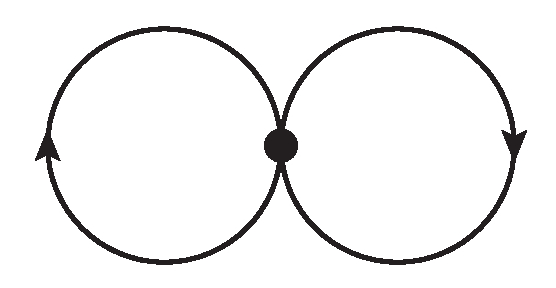
\includegraphics[width=0.1\textwidth, valign=c]{figurer/feynman-diagram/phi-4_loop_notext.eps}
    \times
    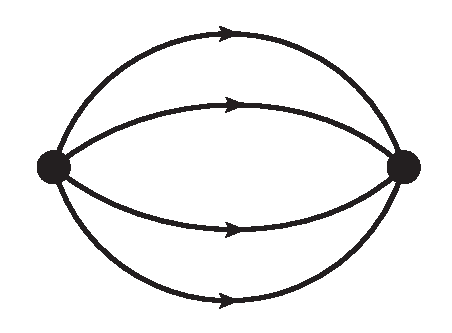
\includegraphics[width=0.08\textwidth, valign=c]{figurer/feynman-diagram/phi-4_2_loop.eps}
    \times
    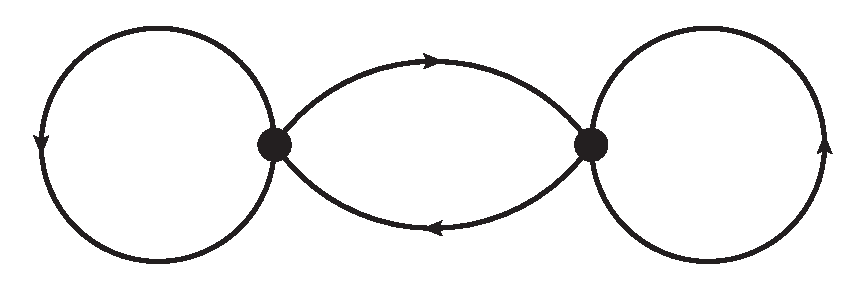
\includegraphics[width=0.14\textwidth, valign=c]{figurer/feynman-diagram/phi-4_2_loop2.eps}
    \times
    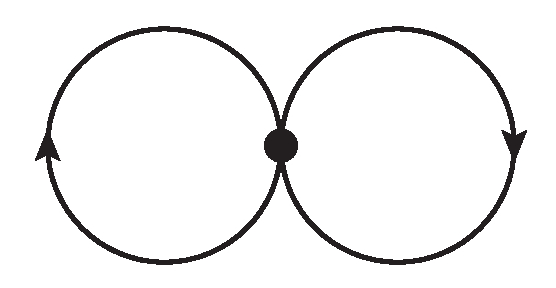
\includegraphics[width=0.1\textwidth, valign=c]{figurer/feynman-diagram/phi-4_loop_notext.eps}
    \times \dots.
\end{align}
If the value of sub diagram $i$ is $V_i$, then each copy of that sub diagram contribute a factor $V_i$ to the value of the total diagram.
However, due to the symmetry of permuting identical sub diagrams, one must divide by the extra symmetry factor $s = n_i !$, which is the total number of permutation of all the copies of diagram $i$.
The value of the total diagram is therefore
\begin{align}
    \label{Feynman diagrams}
    V
    = \prod_{i= 1}^N \frac{1}{n_i!} V_i^{n_i}.
\end{align}
$V$ is uniquely defined by a finite sequence of integers, $(n_1, n_2, \dots n_N, 0, 0, \dots)$, so the sum of all diagrams is the sum over the set $S$ of all finite integers.
This allows us to write the sum of all diagrams as
\begin{equation}
    \label{sum of all diagrams}
    \sum_{(n_1, ...)\in S} \prod_{i} \frac{1}{n_i!} V_i^{n_i}
    = \prod_{i = 1}^{\infty} \sum_{n_i=1}^{\infty} \frac{1}{n_i!} V_i^{n_i}
    = \exp(i {\sum}_i V_i).
\end{equation}

In a free theory, we are able to write
\begin{equation}
    Z_0[J] = Z_0[0] \exp(i W_0[J]), \quad 
    W_0[J] = \frac{1}{2} \int \dd^4 x \dd^4 y \, J(x) D_0(x - y) J(y),
\end{equation}
where $D_0$ is the propagator of the free theory.
The exponential form of $Z[J]$ leads to Wick's theorem, which states that an expectation value of $2n$ fields is a sum of \emph{all possible, distinct} combination of $n$ propagators.
To write this in a formal way, we define the functions $a$ and $b$, which define a way to pair up $2m$ elements.
The domain of the functions are the integers between $1$ and $m$, the image a subset of the integers between $1$ and $2m$ of size $m$.
A valid pairing is a set $\{(a(1), b(1)), \dots (a(m), b(m))\}$, where all elements $a(i)$ and $b(j)$ are different, such all integers up to and including $2m$ are featured.
A pair is not directed, so $(a(i), b(i))$ is the same pair as $(b(i), a(i))$.
Wick theorem states that,
\begin{equation}
    \ex{{\prod}_{i=1}^{2m} \varphi(x_i)  }_0
    = \sum_{\{(a, b)\}} \ex{\varphi(x_{a(i)}) \varphi(x_{b(i)})}_0,
\end{equation}
where the sum is over all tuples $(a, b)$ that define a valid and unique pairing.

Finally, the generating functional $Z[J] = Z[0]\ex{\exp(i \int \dd x \, J \varphi)} $ is the sum of all diagrams with any number of external sources, $J$. 
Using \autoref{sum of all diagrams}, we can write
\begin{equation}
    Z[J] = Z[0] \exp(i W[J]),
\end{equation}
where $W[J]$ is the sum of all \emph{connected} diagrams with external sources.
Finally, using \autoref{correlator from generating functional}, 
\begin{equation}
    \ex{\varphi(x_1)\varphi(x_2)...}
    = 
\end{equation}

% Here we defined the \emph{generating functional for connected diagrams}, $W[J]$.
% The reason for the name will become apparent later. (HUSK Å REFFERE TILBAKE)
% The expectation value of some function of the field-configuration, $A = A[\varphi]$, in the precesense of the source $J$ is
% \begin{equation}
%     \ex{A}_J = \frac{1}{Z[J]} A\left( -i  \fdv{J}\right) Z[J].
% \end{equation}
% (DEFINE FUNCTIONAL DERIVATIVE)
% The expectation value of the field defines a functional,
% \begin{equation}
%     \label{calssical field functional}
%     \varphi[J](x) = \ex{\varphi(x)}_J = 
%     \frac{1}{Z[J]} \left( -i  \fdv{J}\right) Z[J]
%     = \fdv{J(x)} W[J],
% \end{equation}
% and is sometimes called the \emph{classical field}.
% The notation $\Ef[f](x)$ means that $\Ef$ is a functional which takes in a function $f$, and returns the new function $(\Ef[f])(x)$.
% One example is the Lagrangian density, which takes in a field, and returns a function which has a value for each point in space-time.
% We can reverse this relationship, by defining the functional $J[\varphi](x)$ as \emph{the current which causes the classical field $\varphi$}.
% That is, if $\varphi[J_0](x) = \varphi_0(x)$ for some source $J_0$, then $J[\varphi_0] = J_0$

We can use the Legendre-transformation of $W[J]$ to define the new quantity,
\begin{equation}
    \Gamma[\varphi]
    = W[J] - \int \dd x \, J(x) \varphi(x), 
\end{equation}
such that
\begin{equation}
    \fdv{\varphi(x)} \Gamma[\varphi]
    = \int \dd y \, \fdv{J(y)}{\varphi(x)} \fdv{J(y)} W[J]
    - \int \dd y \, \fdv{J(y)}{\varphi(x)} \varphi(x)
    - J(x)
    = - J(x).
\end{equation}
Here, we used the relation \autoref{calssical field functional}.
This means that the equations of motion for the expectation value of the field in the absence of an external current is
\begin{equation}
    \fdv{\Gamma}{\varphi} = 0.
\end{equation}
This is similar to the classical Euler-Lagrange equations, which are
Comparing this to the classical Euler-Lagrange equations with a source,
\begin{equation}
    \fdv{S}{\varphi} = \pdv{\Ell}{\pi} - \partial_\mu \pdv{\Ell}{(\partial_\mu \varphi)} = 0,
\end{equation}
we see that the effective potential $\Gamma$
and is why $\Gamma$ is called the \emph{effective potential}.

In free theory, we may write
\begin{equation}
    W[J] = \frac{1}{2} \int \dd^x \dd^4y J(x) D_0(x - y) J(y),
\end{equation}
where $D_0$ is the free propagator.
We may reverse the relation \autoref{calssical field functional} to write the source in terms of the field,
\begin{equation}
    J = D_0^{-1} \varphi(x)
\end{equation}
This is the field equation for the free field with a source.
For the scalar Klein-Gordon field, $D_0^{-1} = \partial^2 + m^2$
Inserting these two relation into the definition of the effective action, and assuming we can do partial integration with $D_0^{-1}$, we get
\begin{equation}
    \Gamma[\varphi] = W[J] - \int \dd^4x J(x)\varphi(x)
    = 
    \int \dd x( 
        \frac{1}{2}\int \dd y (D_0^{-1} \varphi ) D_0 (D_0^{-1} \varphi ) 
        - (D_0^{-1} \varphi ) \varphi
        )
    = - \frac{1}{2} \int \dd^4 x \varphi(x) D_0^{-1} \varphi(x)
\end{equation}
This is the classical action.
Thus, the effective action $\Gamma$ and the classical action $S$ are the same to first order in perturbation theory.

To interpret $\Gamma$ further, we can define a new theory, with a coupling $g$, 
\begin{equation}
    \label{partition function with g}
    Z[J, g] = \int \D \varphi 
    \exp{ i g^{-1} \left( \Gamma[\varphi] + \int \dd^4x \varphi(x) J(x) \right) }
    = e^{iW[J]}
\end{equation}
The propagator for this theory is 
\begin{equation}
    D_g(x - y) 
    =
    \left(
         - g^{-1} \frac{\delta^2 \Gamma}{\delta \varphi(x) \delta \varphi(y)} 
         \right)^{-1} \propto g
\end{equation}
All vertices in this theory, on the other hand, will be proportional to $g^{-1}$.
Regardless of what the Feynman-diagrams in this theory are, the number of loops of a connected diagram is $L = V - I + 1$, where $V$ is the number of vertices, and $I$ the number of internal lines.
To see this, one can imagine adding a new vertex to an existing diagram.
This splits a line in two.
Any line stemming from this vertex that connect back into the same diagram, create the same number of new loops, vertices and lines, and the formula is fulfilled by induction.
This means that any diagram is proportional to $g^{L+1}$.
In the limit $g \rightarrow 0$, the theory is fully described by only three-level diagrams.
Furthermore, we may use the stationary approximation on \autoref{partition function with g}.
In one dimension, it is given by
\begin{equation}
    \int \dd x \, \exp(i g f(x)) 
    \approx \sqrt{\frac{2 \pi }{f''(x_0)}}\exp( f(x_0)), 
    \, f'(x) = 0, g\rightarrow \infty
\end{equation}
The generalization of this approximation gives
\begin{equation}
    Z \approx 
    C \det(- \frac{\delta^2 \Gamma[\varphi']}{\delta \varphi^2})
    \exp{i g^{-1} \left(\Gamma[\varphi'] + \int \dd^4x J \varphi'  \right)  },
\end{equation}
where $\varphi'$ fulfills
\begin{equation}
    \funcdv{\varphi} \left( \Gamma[\varphi] + \int \dd^4 x J \varphi \right)
    = \funcdv{\varphi(x)}{\Gamma} + J(x) = 0,
\end{equation}
which is exactly $\varphi[J](x)$. This means that
\begin{equation}
    g W[J] = \Gamma[\varphi] + \int \dd^4x\,  J(x) \varphi(x) + \mathcal{O}(g)
\end{equation}


Let $\varphi^*$ solve the quantum mechanical version of the equation of motion, i.e.
\begin{equation}
    \fdv{\Gamma[\varphi^*]}{\varphi} = 0.
\end{equation}
We can Taylor-expand the classical action around this point, by setting $\varphi(x) = \varphi^*(x) + \eta(x)$ for some function $\eta$.
The generating functional becomes
\begin{align}
    Z[J] 
    = \int \D (\varphi^* + \eta) \, 
    \exp{i S[\varphi^* + \eta] + i \int \dd^4 x J (\varphi^* + \eta) }
\end{align}
The functional version of a Taylor expansion is
\begin{equation}
    S[\varphi^* + \eta] = 
    S[\varphi^*]
    + \int \dd x \fdv{S[\varphi^*]}{\varphi(x)} \eta(x)
    + \frac{1}{2} \int \dd x \dd y\,  \frac{\delta^2 S[\varphi^*]}{\delta\varphi(x)\delta\varphi(y)} \eta(x) \eta(y)
    + \dots
\end{equation}
Inserting this into $Z[J]$, with $S_I$ to denote the derivatives of higher order than $2$, we get
\begin{align*}
    &Z[J] = \\ 
    &\int \D \eta  
    \exp{
        i \int \dd^4 x \left(  \Ell[\varphi^*] + J \varphi^*  \right)
        + i \int \dd x \left(  \fdv{S[\varphi^*]}{\varphi(x)} + J(x) \right) \eta(x)
        + i \frac{1}{2} \int \dd x \dd y\,  
        \frac{\delta^2 S[\varphi^*]}{\delta\varphi(x)\delta\varphi(y)} \eta(x) \eta(y) 
        + i S_I[\eta]
        }
\end{align*}
In the first term we used the definition of the classical action. This term is constant with respect to $\eta$, and may therefore be taken outside the path integral.
The next term is the calssical eqation of motion with a source, 
\begin{equation}
    \fdv{S[\varphi]}{\varphi(x)} = - J(x),
\end{equation} 
evaluated at $\varphi^*$.
\begin{equation}
    \fdv{S[\varphi^*]}{\varphi(x)} + J(x)
    = \fdv{\Gamma[\varphi^*]}{\varphi(x)} + J(x)
    + \left(\fdv{S[\varphi^*]}{\varphi(x)} - \fdv{\Gamma[\varphi^*]}{\varphi(x)} \right)
    = \left(\fdv{S[\varphi^*]}{\varphi(x)} - \fdv{\Gamma[\varphi^*]}{\varphi(x)} \right)
    := \delta J
\end{equation}
The second to last term is a Gaussian integral, and may be evaluated as described in \autoref{gaussian integrals},
\begin{equation}
    \int \D \eta \, \exp(
        i \frac{1}{2} \int \dd x \dd y\,  
        \frac{\delta^2 S[\varphi^*]}{\varphi(x)\varphi(y)} \eta(x) \eta(y)
        )
        = C \det\left( \frac{\delta^2 S[\varphi^*]}{\delta \varphi^2} \right)^{-1/2}
\end{equation}
This leaves us with 
\begin{align}
    \label{generating functional}
    W[J] 
    & = -i \ln(Z) \\
    & = 
    \int\dd^4 x \, \left(\Ell[\varphi^*] + J \varphi^*\right)
    - \frac{1}{2} \Tr{\ln\left( - \frac{\delta^2 S[\varphi^*]}{\delta \varphi^2} \right)}
    + \int \D \eta \, \exp{i \int \dd^4 x \delta J(x) \eta  }
    + \int \D \eta \, e^{iS_I}
\end{align}
$\delta J$ is ultimately dependent on our choice of $J$ to define $\varphi$.
It contributes to the expectation value of $\eta$, through tadpole diagrams
\begin{align}
    \ex{\eta}_{j=0} = 
    \feynmandiagram [horizontal=a to b]{
    a --[inline=(b.base), fermion] b[blob]
    }; 
\end{align}
This can be removed by using the renormalization condition
\begin{equation}
    \feynmandiagram [horizontal=a to b]{
    a --[inline=(b.base), fermion] b[blob]
    };
    = 0.
\end{equation}


\subsection{Minimizing energy}
%%%%%%%%%%%%%%%%%
%%%% SECTION %%%%
%%%%%%%%%%%%%%%%%
The value of $\alpha$ is found by minimizing the free energy. 
The first approximation to the free energy in the ground state is the static part of the Hamiltonian density $\He^{(0)}$, which we get from \autoref{L0} through
\begin{equation}
    \He_2^{(0)} = - \Ell_2^{(0)} = 
    -f^2   
    \left(
        2B_0m \cos{\alpha}
        + \frac{1}{2} \mu^2 \sin^2{\alpha}
    \right),
\end{equation}
The minimum of this function is achieved when
\begin{align*}
    &\dv{\alpha} \He_2^{(0)} 
    = f^2\left(2B_0m - \mu_I^2\cos{\alpha}\right)\sin{\alpha}
    = 0.
\end{align*}
This gives the solution set and minimization criterion
\begin{align}
    \alpha = \pi n, \, n \in \mathbb{Z} \quad
    \mathrm{or} \quad
    \cos{\alpha} = \frac{2B_0m}{\mu_I{}^2}.
\end{align}
We see that the linear part of the potential from \autoref{L1}, $\Ve^{(1)} = f(\mu_I{}^2\cos{\alpha} - 2B_0m)\pi_1 \sin{\alpha}= 0$ if and only if the criterion for minimization is fulfilled.

\subsection{Propagator}
%%%%%%%%%%%%%%%%%
%%%% SECTION %%%%
%%%%%%%%%%%%%%%%%
\label{section:propagator}
We may write the quadratic part of the Lagrangian \autoref{L2} as \footnote{Summation over isospin index ($a,b,c$) will be explicit in this section.}
\begin{align}
    \label{quadratic lagrangian}
    \Ell_2^{(2)}
    =
    \frac{1}{2} \sum_a \partial_\mu \pi_a \partial^\mu \pi_a
    + \frac{1}{2} m_{12} (\pi_1 \partial_0 \pi_2 - \pi_2 \partial_0 \pi_1)
    - \frac{1}{2} \sum_a m_a^2 \pi_a^2,
\end{align}
where
\begin{align}
    m_1^2 &= 2 B_0 m \cos{\alpha} - \mu_I^2 \cos{2\alpha}, \\
    m_2^2 &= 2 B_0 m \cos{\alpha} - \mu_I^2 \cos^2{\alpha}, \\
    m_3^2 &= 2 B_0 m \cos{\alpha} + \mu_I^2 \sin^2{\alpha}, \\
    m_{12} &= 2 \mu_I \cos{\alpha}.
\end{align}
The components of the Euler-Lagrange equations of this field are
\begin{equation*}
    \pdv{\Ell}{\pi_a} = 
    \frac{1}{2} m_{12} (\delta_{a1} \partial_0 \pi_2 - \delta_{a2}\partial_0 \pi_1) 
    - m^2_{a} \pi_a, \quad
    \pdv{\Ell}{(\partial_\mu \pi_a)} = 
    \partial^\mu \pi_a - \frac{1}{2} m_{12} \delta^\mu_0 (\delta_{a1}\pi_2  - \delta_{a2}\pi_1).
\end{equation*}
This gives the equation of motion for the field
\begin{equation}
    \partial^\mu \partial_\mu \pi_a + m_a^2 \pi_a
    =  m_{12}(\delta_{a1} \partial_0 \pi_2  - \delta_{a2} \partial_0 \pi_1).
\end{equation}
The propagator of the pion field is defined by
\begin{equation}
    \left[
        \delta_{ab}(\partial^\mu\partial_\mu + m^2_a)
        -  m_{12}(\delta_{a1} \delta_{b2} - \delta_{a2}\delta_{b1}) \partial_0
    \right] 
    D_{bc}(x, x') 
    = -i \delta(x - x') \delta_{ac}.
\end{equation}
The momentum space propagator, as defined in the \autoref{Conventions and notation}, fulfills
\begin{equation*}
    -\left[
        \delta_{ab}(p^2 - m_a^2)
        +  i p_0 m_{12}(\delta_{a1} \delta_{b2} - \delta_{a2}\delta_{b1}) 
    \right] 
    \tilde D_{bc}(p) 
    := A_{ab} \tilde D_{bc}(p) = -i \delta_{ac},
\end{equation*}
where
\begin{equation*}
    A = -
    \begin{pmatrix}
        p^2 - m^2_1             & i p_0 m_{12}     & 0             \\
        - i p_0 m_{12}            & p^2 - m^2_2       & 0             \\
        0                       & 0                 & p^2 - m^2_3
    \end{pmatrix}.
\end{equation*}
The spectrum of the particles is given by solving $\det(A) = 0$ for $p^0$. With $p = (p_0, P)$ as the four momentum, this gives
\begin{align*}
    \det(A) & = A_{33} \left(A_{11} A_{22} + A_{12}^2\right)
    = - \left(p^2 - m^2_3\right)
    \left[
        \left(p^2 - m^2_1\right)
        \left(p^2 - m^2_2\right)
        - p_0^2 m_{12}^2
    \right] = 0,
\end{align*}
This equation has the solutions
\begin{align}
    E_0^2 &= P^2 + m_2^2, \\
    E_\pm^2
    & = P^2 +
    \frac{1}{2}
    \left(
        m_1^2 + m_2^2 + m_{12}^2 
    \right)
    \pm 
    \frac{1}{2}
    \sqrt{
        4P^2m_{12}^2 
        +
        \left(
            m_1^2 + m_2^2 + m_{12}^2
        \right)^2
        - 4 m_1^2 m_2^2
    }.
\end{align}
This gives the effective masses
\begin{align}
    m_0^2 &= m_2^2, \\
    m_\pm^2
    & =  \frac{1}{2}
    \left[
        m_1^2 + m_2^2 + m_{12}^2 
    \right]
    \pm \frac{1}{2}
    \sqrt{
        \left(
            m_1^2 + m_2^2 + m_{12}^2
        \right)^2
        - 4 m_1^2 m_2^2
    }.
\end{align}
The propagator may then be obtained as described in \autoref{Conventions and notation},
\begin{align}
    \notag
    D_0 & = i A^{-1} = \frac{i}{\det(A)}
    \begin{pmatrix}
        A_{22} A_{33}   & A_{12}A_{33}  & 0 \\
        -A_{12}A_{33}   & A_{11}A_{33}  & 0 \\
        0               & 0             & A_{11}A_{22} + A_{12}^2
    \end{pmatrix} \\
    \label{free pion propagator}
    & = i
    \begin{pmatrix}
        \frac{
            p^2 - m_2^2
        }
        {
            (p_0^2 - E_+^2)(p_0^2 - E_-^2)
        } 
        & \frac{
            - ip_0m_{12}
        }
        {
            (p_0^2 - E_+^2)(p_0^2 - E_-^2)
        } & 0 \\
        \frac{
            ip_0m_{12}
        }
        {
            (p_0^2 - E_+^2)(p_0^2 - E_-^2)
        }
        & \frac{
            p^2 - m_1^2
        }
        {
            (p_0^2 - E_+^2)(p_0^2 - E_-^2)
        } & 0 \\
        0 & 0 & 
        \frac{1}{p_0^2 - E_0^2}
    \end{pmatrix}.
\end{align}
